%% This is file `jasr-template.tex',
%% 
%% Copyright 2019-2020 Elsevier Ltd
%% 
%% This file is part of the 'Elsarticle Bundle'.
%% ---------------------------------------------
%% 
%% It may be distributed under the conditions of the LaTeX Project Public
%% License, either version 1.2 of this license or (at your option) any
%% later version.  The latest version of this license is in
%%    http://www.latex-project.org/lppl.txt
%% and version 1.2 or later is part of all distributions of LaTeX
%% version 1999/12/01 or later.
%% 
%% The list of all files belonging to the 'Elsarticle Bundle' is
%% given in the file `manifest.txt'.
%% 
%% Template article for Elsevier's document class `elsarticle'
%% with harvard style bibliographic references
%%
%% $Id: jasr-template.tex 188 2020-11-16 05:18:23Z rishi $
%%
%% Use the option review to obtain double line spacing
%\documentclass[times,review,preprint,authoryear]{elsarticle}

%% Use the options `twocolumn,final' to obtain the final layout
%% Use longtitle option to break abstract to multiple pages if overfull.
%% For Review pdf (With double line spacing)
%\documentclass[times,twocolumn,review]{elsarticle}
%% For abstracts longer than one page.
%\documentclass[times,twocolumn,review,longtitle]{elsarticle}
%% For Review pdf without preprint line
%\documentclass[times,twocolumn,review,nopreprintline]{elsarticle}
%% Final pdf
\documentclass[times,twocolumn,final,authoryear]{elsarticle}
%%
%\documentclass[times,twocolumn,final,longtitle]{elsarticle}
%%

%%
%% Stylefile to load JASR template
\usepackage{jasr}
\usepackage{framed,multirow}

%% The amssymb package provides various useful mathematical symbols
\usepackage{amssymb}
\usepackage{latexsym}

%% For line numbers
%\usepackage[switch]{lineno}

% Following three lines are needed for this document.
% If you are not loading colors or url, then these are
% not required.
\usepackage{url}
\usepackage{xcolor}
\usepackage{multirow}
%\usepackage{tablefootnote}
\definecolor{newcolor}{rgb}{.8,.349,.1}

\usepackage[citebordercolor=white]{hyperref}
\usepackage{rotating}
\usepackage{pdflscape}
\usepackage{longtable}
\journal{Advances in Space Research}

\begin{document}

\verso{Given-name Surname \textit{etal}}

\begin{frontmatter}

\title{Ionospheric Disturbances in Mexican Territory Produced by Objects Entering the Athmosphere from Space \tnoteref{tnote1}}%
%\tnotetext[tnote1]{This is an example for title footnote coding.}

\author[1]{Jorge \snm{Tarango-Yong}\corref{cor1}}
\cortext[cor1]{Tel.: +52-443-476-5525;  \\
  email: jorge.tarango@comunidad.unam.mx
}

\author[1]{Mario \snm{Rodriguez-Martinez}\corref{cor2}}
\cortext[cor2]{email: m.rodriguez@enesmorelia.unam.mx}
%\fntext[fn1]{This is author footnote for second author.}
\author[1]{Raul \snm{Guti\'errez-Zalapa}\fnref{fn1}}
%% Third author's email
%\ead{author3@author.com}
%\author[2]{Given-name4 \snm{Surname4}}

\address[1]{Escuela Nacional de Estudios Superiores, UNAM, campus Morelia, Antigua Carretera a P\'atzcuaro No. 8701
Col. Ex Hacienda de San Jos\'e de la Huerta, Morelia, Michoac\'an, 58190, M\'exico}
%\address[2]{}

\received{1 May 2013}
\finalform{10 May 2013}
\accepted{13 May 2013}
\availableonline{15 May 2013}
\communicated{S. Sarkar}


\begin{abstract}
%%%
Please type your abstract here, and the rest of the text, figures,
tables, equations etc. in the main body. Please do not modify LaTeX\ 
commands unless you need to modify them and know how to do it.
%%%%
\end{abstract}

\begin{keyword}
%% MSC codes here, in the form: \MSC code \sep code
%% or \MSC[2008] code \sep code (2000 is the default)
%\MSC 41A05\sep 41A10\sep 65D05\sep 65D17
%% Keywords
\KWD Space Sciences\sep Atmosphere%\sep Keyword3
\end{keyword}

\end{frontmatter}

%% For linenumbers
%\linenumbers

%% main text
\section{Introduction}
\label{sec1}
%Please use \verb+elsarticle.cls+ for typesetting your paper. Additionally,
%make sure not to remove the package \verb+jasr.sty+ already included in the
%preamble:
%\begin{verbatim} 
%  \usepackage{jasr}
%\end{verbatim}

%Make sure to have the file \verb+model5-names.bst+ to produce the references in
%the correct format. 

%Any instructions relevant to the \verb+elsarticle.cls+ are
%applicable here as well. See the online instruction available at:
%\makeatletter
%\if@twocolumn
%\begin{verbatim}
% https://support.stmdocs.in/wiki/
% index.php?title=Elsarticle.cls
%\end{verbatim}
%\else
%\begin{verbatim}
% https://support.stmdocs.in/wiki/index.php?title=Elsarticle.cls
% \end{verbatim}
%\fi
%\makeatother

%Following commands are defined for this journal which are not in
%\verb+elsarticle.cls+. 
%\begin{verbatim}
%  \received{}
%  \finalform{}
%  \accepted{}
%  \availableonline{}
%  \communicated{}
%\end{verbatim}


%\subsection{Subsection}
%This is only a \LaTeX\ template if you need one. 
%See the detailed guidelines for manuscript preparation 
%and submission at:
%\begin{verbatim}
%https://ees.elsevier.com/asr
%\end{verbatim}


\section{Metodology}
\subsection{Meteors Database}

We selected a sample of meteors which were observed in mexican territory from the Geostationary Lightning Mapper \citep{GOODMAN:2013}. Orignally this project was designed to detect ligthning activity in earth's athmosphere, but has been proven that also can detect bolides entering the athmosphere. The detection comes from two satellites called GOES-16 and GOES-17 orbiting the earth in geostationary orbits. We used the interactive database available at \url{https://neo-bolide.ndc.nasa.gov/#/} to get the events positions presented in this section, as well we obtained data about the bolid trajectory detected and energy released. The sample was chosen following the next criteria:%selected in such way we chose the most probable objects to be detected by GPS sources in mexican territory and its surroundings: 

\begin{itemize}
    \item The objects were detected inside mexican territory and its surroundings.
    \item The objects were detected by both satellites GOES 16 and GOES 17 (stereo)
    \item The detection has been assigned a high confidence ratio.
\end{itemize}



 



\begin{table*}
  \centering
  \caption{List of meteors passing through Mexico. The events are listed in chronological order. The listed duration, latitude and longitude correspond to the mean of the measurements of both GOES satellites. The uncertainties correspond to the respecting mean deviation.}
\label{tab:table-meteors}
\begin{tabular}{rrrrrr}
\hline
ID & Date of event & Start Time (UT)  & Duration (seconds) & Latitude (deg) & Longitude (deg)\\
\hline
01 & 2019-05-23 & 16:36:18 & $0.197\pm 0.0000$ & $24.30 \pm 0.000$ & $-101.60 \pm 0.849$\\
02 & 2019-07-18 & 14:30:30 & $0.058\pm 0.0000$ & $27.20 \pm 0.000$ & $-103.15 \pm 0.778$\\
03 & 2019-08-10 & 11:18:48 & $0.199\pm 0.0757$ & $21.50 \pm 0.000$ & $-102.50  \pm 0.849$\\
04 & 2019-10-03 & 07:55:33 & $0.106\pm 0.0297$ & $25.65 \pm 0.071$ & $-96.25 \pm   0.778$\\
05 & 2019-10-09 & 06:08:11 & $0.103\pm 0.0078$ & $23.60 \pm 0.000$ & $-111.95 \pm  0.212$\\
06 & 2019-11-16 & 09:36:04 & $0.396\pm 0.0134$ & $20.30 \pm 0.000$ & $-100.55 \pm  0.919$\\
07 & 2019-11-17 & 15:36:01 & $0.116\pm 0.0035$ & $31.70 \pm 0.000$ & $-117.70 \pm  1.131$\\
08 & 2019-11-19 & 07:57:40 & $0.097\pm 0.1138$ & $20.00 \pm 0.000$ & $-88.40 \pm  1.131$\\
09 & 2019-11-26 & 13:23:20 & $0.078\pm 0.0290$ & $23.90 \pm 0.000$ & $-108.70 \pm  0.849$\\
10 & 2019-12-04 & 09:42:54 & $0.173\pm 0.0028$ & $31.50 \pm 0.000$ & $-113.65 \pm  0.919$\\
11 & 2019-12-15 & 14:50:49 & $0.127\pm 0.0134$ & $27.70 \pm 0.000$ & $-114.10 \pm  0.849$\\
12 & 2019-12-29 & 16:16:35 & $0.062\pm 0.0134$ & $29.60 \pm 0.000$ & $-116.35 \pm  0.919$\\
13 & 2020-01-03 & 14:10:17 & $0.113\pm 0.0085$ & $30.20 \pm 0.000$ & $-117.65 \pm  0.919$\\
14 & 2020-01-06 & 16:39:27 & $0.118\pm 0.0042$ & $31.40 \pm 0.000$ & $-108.20 \pm  0.990$\\
15 & 2020-01-15 & 15:00:33 & $0.213\pm 0.1351$ & $19.45 \pm 0.071$ & $-95.55 \pm   0.919$\\
16 & 2020-02-12 & 09:25:40 & $0.210\pm 0.0226$ & $18.90 \pm 0.000$ & $-93.50 \pm   0.849$\\
17 & 2020-03-03 & 12:33:27 & $0.062\pm 0.0007$ & $18.25 \pm 0.071$ & $-106.35 \pm 0.636$\\
18 & 2020-03-31 & 19:31:52 & $0.105\pm 0.0573$ & $28.45 \pm 0.071$ & $-112.05 \pm  0.636$\\
19 & 2020-04-08 & 16:25:28 & $0.120\pm 0.0926$ & $26.10 \pm 0.000$ & $-93.90 \pm   0.849$\\
20 & 2020-04-18 & 17:43:25 & $0.139\pm 0.0106$ & $29.00 \pm 0.000$ & $-106.55 \pm  0.919$\\
21 & 2020-04-20 & 16:05:22 & $0.318\pm 0.1655$ & $28.15 \pm 0.071$ & $-97.85 \pm   1.061$\\
22 & 2020-04-25 & 11:03:09 & $0.323\pm 0.0813$ & $32.15 \pm 0.071$ & $-111.60 \pm  1.131$\\
23 & 2020-04-28 & 19:31:52 & $0.105\pm 0.0573$ & $28.45 \pm 0.071$ & $-112.05 \pm  0.636$\\
24 & 2020-05-08 & 10:06:16 & $0.490\pm 0.0750$ & $21.60 \pm 0.000$ & $-92.40 \pm   0.849$\\
25 & 2020-07-15 & 19:58:28 & $0.693\pm 0.0495$ & $24.00 \pm 0.000$ & $-108.35 \pm  0.495$\\
26 & 2020-08-07 & 13:29:57 & $0.163\pm 0.0057$ & $28.80 \pm 0.000$ & $-106.05 \pm  0.919$\\
27 & 2020-09-13 & 16:41:59 & $0.184\pm 0.0078$ & $28.45 \pm 0.071$ & $-113.75 \pm  0.919$\\
28 & 2020-09-30 & 12:28:11 & $0.100\pm 0.0078$ & $24.90 \pm 0.000$ & $-110.90 \pm  0.849$\\
29 & 2020-11-16 & 12:28:11 & $0.100\pm 0.0078$ & $24.90 \pm 0.000$ & $-110.90 \pm  0.849$\\
30 & 2020-11-17 & 12:53:41 & $0.404\pm 0.0262$ & $23.00 \pm 0.000$ & $-102.45 \pm  0.919$\\
31 & 2020-12-19 & 10:18:14 & $0.407\pm 0.0110$ & $21.95 \pm 0.071$ & $-101.60 \pm  0.990$\\
32 & 2020-12-23 & 09:43:01 & $0.148\pm 0.0014$ & $25.75 \pm 0.071$ & $-111.25 \pm  0.778$\\
33 & 2020-12-29 & 15:20:54 & $0.118\pm 0.0014$ & $16.80 \pm 0.000$ & $-102.20 \pm  0.707$\\
34 & 2021-03-31 & 09:01:17 & $0.753\pm 0.3083$ & $20.15 \pm 0.071$ & $-92.95 \pm  0.212$\\\hline
\end{tabular}
\end{table*}

\begin{figure}
  \centering
  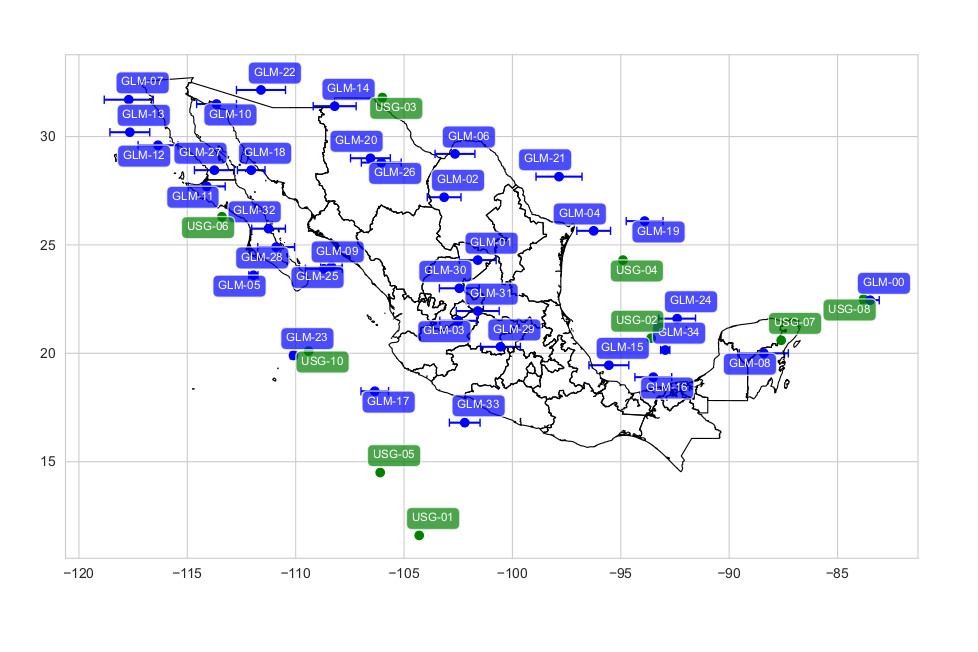
\includegraphics[width=\linewidth]{../meteors_map}
  \caption{Positions of events from table \ref{tab:table-meteors}. The label of each point correspond to the ID (first column) of the referred table.}
  \label{fig:meteors-map}
\end{figure}

\subsection{GPS data}

This material is based on services provided by the GAGE Facility, operated by UNAVCO, Inc., with support from the National Science Foundation and the National Aeronautics and Space Administration under NSF Cooperative Agreement EAR-1724794.

We got RINEX data from 3 to 7 stations depending of the event location and data availability that surround the event place in all directions as possible. A list of the stations where we got RINEX data is available in table  . Most of the stations lie in mexican territory, but in some cases we required data from other stations to cover events near the mexican frontier at north or south.

\clearpage
\onecolumn
\begin{landscape}
%\begin{table*}
%    \centering
  \begin{longtable}{lllp{4cm}p{10cm}}
      \caption{List of GPS stations used for this work.}
      \label{tab:table-stations}
      \endfirsthead
      \endhead
    \hline
    Station name & Latitude & Longitude & Date of events  & Citation \\\hline
    BAR1\hyperlink{Hudnut}{${}^1$}\hyperlink{Hudnut2}{${}^5$}& 33.48 & -119.03 & 2019-12-29 2020-01-03 & UNAVCO Community, Hudnut, Kenneth, King, Nancy, Aspiotes, Aris G., Borsa, Adrian A., Determan, Daniel N., Galetzka, John E., Stark, Keith F., 2005, SCIGN-PBO Nucleus GPS Network - BAR1-Santa Barbara Island One P.S., The GAGE Facility operated by UNAVCO, Inc., GPS/GNSS Observations Dataset, \url{https://doi.org/10.7283/T5668BHN}.\\
    BLYT\hyperlink{Hudnut}{${}^1$} & 33.61 & -114.71 & 2019-12-29 2020-01-03 & Hudnut, Kenneth, King, Nancy, Aspiotes, Aris G., Borsa, Adrian A., Determan, Daniel N., Galetzka, John E., Stark, Keith F., 2006, SCIGN USGS GPS Network - BLYT-Blythe P.S., The GAGE Facility operated by UNAVCO, Inc., GPS/GNSS Observations Dataset, \url{https://doi.org/10.7283/T5HT2MKK}.\\
    CN23 & 17.26 & -88.78 & 2019-11-19 2020-01-15 2020-02-12& UNAVCO Community, 2012, COCONet GPS Network - CN23-BelmopanBZCR2012 P.S., The GAGE Facility operated by UNAVCO, Inc., GPS/GNSS Observations Dataset, \url{https://doi.org/10.7283/T5Q23XJH}.\\
    CN25 & 16.23 & -92.13 & 2020-01-15 & UNAVCO Community, 2014, COCONet GPS Network - CN25-ComitandDMEX2012 P.S., The GAGE Facility operated by UNAVCO, Inc., GPS/GNSS Observations Dataset, \url{https://doi.org/10.7283/T57W69G7}.\\
    GCFS & 19.31 & -81.18 & 2019-11-19& Watts, Anthony, 2016, COCONet GPS Network - GCFS-G\_CAYMAN\_CYM2014 P.S., The GAGE Facility operated by UNAVCO, Inc., GPS/GNSS Observations Dataset, \url{https://doi.org/10.7283/7ETV-X536}.\\
    GMPK\hyperlink{Hudnut}{${}^1$} & 33.05 & -114.83 & 2019-12-04 & UNAVCO Community, Hudnut, Kenneth, King, Nancy, Aspiotes, Aris G., Borsa, Adrian A., Determan, Daniel N., Galetzka, John E., Stark, Keith F., 2005, SCIGN-PBO Nucleus GPS Network - GMPK-Glamis Peak P.S., The GAGE Facility operated by UNAVCO, Inc., GPS/GNSS Observations Dataset, \url{https://doi.org/10.7283/WCHN-H687}.\\
    GUAT\hyperlink{Garnier}{${}^2$} & 14.59 & -90.52 & 2020-02-12 & DeMets, Charles, Cosenza-Muralles, Beatriz, 2021, Central America 2018 - Guatemala, The GAGE Facility operated by UNAVCO, Inc., GPS/GNSS Observations Dataset, \url{https://doi.org/10.7283/KH2R-K704}.\\
    GUAX\hyperlink{Hudnut}{${}^1$} & 28.88 & -118.29 & 2019-10-09 2019-12-15 2019-12-29 2020-01-03 2020-03-31 2020-07-15 2020-09-13 2020-09-30 2020-12-23 & Hudnut, Kenneth, King, Nancy, Aspiotes, Aris G., Borsa, Adrian A., Determan, Daniel N., Galetzka, John E., Stark, Keith F., 2001, SCIGN USGS GPS Network - GUAX-Isla Guadalupe P.S., The GAGE Facility operated by UNAVCO, Inc., GPS/GNSS Observations Dataset, \url{https://doi.org/10.7283/T5GX48T2}.\\
    IAGX & 29.03 & -113.17 & 2019-12-04 & Gonzalez-Ortega, Alejandro, Galetzka, John E., Gonzalez, Javier, 2018, CICESE REGNOM GPS Network - IAGX-iagxREGNOMmx2018 P.S., The GAGE Facility operated by UNAVCO, Inc., GPS/GNSS Observations Dataset, \url{https://doi.org/10.7283/DGWN-A627}.\\
    INEG & 21.85 & -102.28 & 2020-07-15 2020-08-07 2020-09-30 2020-11-16 2020-11-17 2020-12-19 & No citations were found\\
    KVTX & 27.55 & -97.89 & 2019-05-23 2019-07-18 2019-08-10 2019-10-03 2019-11-17 2020-04-08 2020-04-18 2020-04-20 2020-05-08 2020-08-07 & UNAVCO Community, 2007, PBO GPS Network - KVTX-KingsvilleTX2006 P.S., The GAGE Facility operated by UNAVCO, Inc., GPS/GNSS Observations Dataset, \url{https://doi.org/10.7283/T5J38QH8}.\\
    MDO1 & 30.68 & -104.02 & 2019-07-18& No citations were found\\
    MGO5 & 30.68 & -104.02 & 2020-04-20 2020-08-07 & No citations were found\\
    MGW3 & 29.62 & -89.95 & 2020-04-08 2020-04-20 2020-05-08 & No citations were found\\
    OXTH & 16.29 & -95.24 & 2020-01-15 2020-02-12 & DeMets, Charles, Cabral-Cano, Enrique, 2008, Oaxaca GPS Network - OXTH-Tehuantepec P.S., The GAGE Facility operated by UNAVCO, Inc., GPS/GNSS Observations Dataset, \url{https://doi.org/10.7283/T5Q81B5V}.\\
    OXUM\hyperlink{Graham}{${}^3$} & 15.66 & -96.50 & 2021-03-31 & Cabral-Cano, Enrique, Salazar-Tlaczani, Luis, 2015, TLALOCNet - OXUM-oxum\_tnet\_mx2001 P.S., The GAGE Facility operated by UNAVCO, Inc., GPS/GNSS Observations Dataset, \url{https://doi.org/10.7283/T5J964RP}.\\
    P001 & 31.95 & -112.80 & 2020-04 25 & UNAVCO Community, 2008, PBO GPS Network - P001-Organ\_PipeAZ2007 P.S., The GAGE Facility operated by UNAVCO, Inc., GPS/GNSS Observations Dataset, \url{https://doi.org/10.7283/T5DR2SGP}.\\
    P014 & 31.97 & -11.09 & 2019-12-04 2019-12-29 2020-01-03 2020-01-06 2020-04-25 & UNAVCO Community, 2008, PBO GPS Network - P014-Sahuarita\_AZ2007 P.S., The GAGE Facility operated by UNAVCO, Inc., GPS/GNSS Observations Dataset, \url{https://doi.org/10.7283/T5DJ5CMK}.\\
    P807 & 30.49 & -98.82 & 2019-11-17 2020-01-06 2020-04-20 2020-11-17 & UNAVCO Community, 2012, PBO GPS Network - P807-EcRockStPkTX2012 P.S., The GAGE Facility operated by UNAVCO, Inc., GPS/GNSS Observations Dataset, \url{https://doi.org/10.7283/T5TQ5ZKM}.\\
    PLPX & 31.59 & -115.15 & 2019-12-04 & UNAVCO Community, 2011, PBO GPS Network - PLPX-Las\_PintasMX2010 P.S., The GAGE Facility operated by UNAVCO, Inc., GPS/GNSS Observations Dataset, \url{https://doi.org/10.7283/T5K64G3T}.\\
    PTEX & 32.29 & -116.52 & 2019-12-29 2020-01-03 2020-09-13 2020-12-23 & UNAVCO Community, 2011, PBO GPS Network - PTEX-Testerazo\_MX2011 P.S., The GAGE Facility operated by UNAVCO, Inc., GPS/GNSS Observations Dataset, \url{https://doi.org/10.7283/T5610XBP}.\\
    RG06 & 32.63 & -107.86 & 2020-04-25 & Sheehan, Anne, 2007, Rio Grande Rift GPS Network - RG06-RG06FaywodNM2006 P.S., The GAGE Facility operated by UNAVCO, Inc., GPS/GNSS Observations Dataset, \url{https://doi.org/10.7283/T5668BFR}.\\
    RG07 & 32.50 & -106.84 & 2020-01-06 & Sheehan, Anne, 2007, Rio Grande Rift GPS Network - RG07-RG07CrucesNM2006 P.S., The GAGE Facility operated by UNAVCO, Inc., GPS/GNSS Observations Dataset, \url{https://doi.org/10.7283/T5KD1W45}. \\
    SG33 & 31.77 & -106.51 & 2019-11-17 2020-04-18 2020-08-07 & Harder, Steven, Kaip, Galen, Montana, Carlos, 2004, SuomiNet-G GPS Network - SG33-UTEP P.S., The GAGE Facility operated by UNAVCO, Inc., GPS/GNSS Observations Dataset, \url{https://doi.org/10.7283/T50863KQ}.\\
    TGMX  & 20.87 & -86.87 & 2021-03-31 & UNAVCO Community, 2015, COCONet GPS Network - TGMX-PtoMor\_TG\_MX2015 P.S., The GAGE Facility operated by UNAVCO, Inc., GPS/GNSS Observations Dataset, \url{https://doi.org/10.7283/T5154FB7}.\\
    TNAM & 20.54 & -103.97 & 2020-03-03 2020-07-15 2020-09-30 2020-11-16 2020-11-17 2020-12-19 & UNAVCO Community, 2014, TLALOCNet - TNAM-TNAM\_TNET\_MX2014 P.S., The GAGE Facility operated by UNAVCO, Inc., GPS/GNSS Observations Dataset, \url{https://doi.org/10.7283/T5QF8R4R}.\\
    TNAT & 18.13 & -98.04 & 2020-01-15 & UNAVCO Community, 2014, TLALOCNet - TNAT-TNAT\_TNET\_MX2014 P.S., The GAGE Facility operated by UNAVCO, Inc., GPS/GNSS Observations Dataset, \url{https://doi.org/10.7283/T5G15Z4S}.\\
    TNBA & 28.97 & -113.55 & 2019-10-09 2019-11-26 2019-12-15 2019-12-29 2020-01-03& UNAVCO Community, 2015, TLALOCNet - TNBA-TNBA\_TNET\_MX2014 P.S., The GAGE Facility operated by UNAVCO, Inc., GPS/GNSS Observations Dataset, \url{https://doi.org/10.7283/T57M0688}.\\
    TNCC & 18.79 & -103.17 & 2020-03-03 & UNAVCO Community, 2015, TLALOCNet - TNCC-TNCC\_TNET\_MX2015 P.S., The GAGE Facility operated by UNAVCO, Inc., GPS/GNSS Observations Dataset, \url{https://doi.org/10.7283/T50R9MSK}.\\
    TNCM & 19.50 & -105.04 & 2020-03-03 2020-04-28 & UNAVCO Community, 2014, TLALOCNet - TNCM-TNCM\_TNET\_MX2014 P.S., The GAGE Facility operated by UNAVCO, Inc., GPS/GNSS Observations Dataset, \url{https://doi.org/10.7283/T5B856FW}.\\
    TNCN & 18.55 & -101.97 & 2020-11-16 2020-12-29 & UNAVCO Community, 2016, TLALOCNet - TNCN-TNCN\_TNET\_MX2016 P.S., The GAGE Facility operated by UNAVCO, Inc., GPS/GNSS Observations Dataset, \url{https://doi.org/10.7283/T5610XQM}.\\
    TNCU & 28.45 & -106.79 & 2019-05-23 2019-07-18 2019-08-10 2019-11-17 2019-12-15 2020-01-06 2020-03-31 2020-04-18 2020-07-15 2020-08-07 2020-11-17 2020-12-19 & UNAVCO Community, 2014, TLALOCNet - TNCU-CuauhtemocTN2014 P.S., The GAGE Facility operated by UNAVCO, Inc., GPS/GNSS Observations Dataset, \url{https://doi.org/10.7283/T5V69GV2}.\\
    TNGF & 19.33 & -99.18 & 2020-11-16 2020-12-29 & Cabral-Cano, Enrique, Salazar-Tlaczani, Luis, 2016, TLALOCNet GPS Network - TNGF\_Geofisica-UNAM\_Mexico\_City\_TNET\_mx2015 P.S., The GAGE Facility operated by UNAVCO, Inc., GPS/GNSS Observations Dataset, \url{https://doi.org/10.7283/T53X851M}.\\
    TNHM & 29.08 & -110.97 & 2019-10-09 2019-11-26 2019-12-04 2019-12-15 2019-12-29 2020-01-03 2020-03-31 2020-04-18 2020-07-15 2020-08-07 2020-09-13 2020-09-30 2020-12-23 & UNAVCO Community, 2014, TLALOCNet - TNHM-hermosilloTN2014 P.S., The GAGE Facility operated by UNAVCO, Inc., GPS/GNSS Observations Dataset, \url{https://doi.org/10.7283/T5KP80FV}.\\
    TNMS & 20.53 & -104.80 & 2019-10-09 2019-11-26 2019-12-15 2020-03-03 2020-07-15 & UNAVCO Community, 2014, TLALOCNet - TNMS-TNMS\_TNET\_MX2014 P.S., The GAGE Facility operated by UNAVCO, Inc., GPS/GNSS Observations Dataset, \url{https://doi.org/10.7283/T56H4FQ5}.\\
    TNNP & 16.12 & -97.14 & 2020-04-28 & Cabral-Cano, Enrique, Salazar-Tlaczani, Luis, DeMets, Charles, 2016, TLALOCNet - TNNP-tnnp\_tnet\_mx2015 P.S., The GAGE Facility operated by UNAVCO, Inc., GPS/GNSS Observations Dataset, \url{https://doi.org/10.7283/T5N29V96}.\\
    TNNX & 17.41 & -97.22 & 2020-01-15 2020-02-12 2020-12-29 2021-03-31 & UNAVCO Community, 2014, TLALOCNet - TNNX-TNNX\_TNET\_MX2014 P.S., The GAGE Facility operated by UNAVCO, Inc., GPS/GNSS Observations Dataset, \url{https://doi.org/10.7283/T52R3PZ0}.\\
    TNPP & 31.34 & -113.63 & 2019-12-04 2020-03-31 2020-04-25 & UNAVCO Community, 2015, TLALOCNet - TNPP-TNPP\_TNET\_MX2015 P.S., The GAGE Facility operated by UNAVCO, Inc., GPS/GNSS Observations Dataset, \url{https://doi.org/10.7283/T5CC0Z0M}.\\
    TNSJ & 16.17 & -96.49 & 2020-12-29 & UNAVCO Community, 2016, TLALOCNet - TNSJ-tnsj\_tnet\_mx2015 P.S., The GAGE Facility operated by UNAVCO, Inc., GPS/GNSS Observations Dataset, \url{https://doi.org/10.7283/T59S1PF1}.\\
    TSFX & 30.93 & -114.81 & 2020-09-13 2020-12-23 & Gonzalez-Ortega, Alejandro, Galetzka, John E., Gonzalez, Javier, 2018, CICESE REGNOM GPS Network - TSFX-tsfxREGNOMmx2016 P.S., The GAGE Facility operated by UNAVCO, Inc., GPS/GNSS Observations Dataset, \url{https://doi.org/10.7283/AGEA-2G27}.\\
    UAGU & 21.92 & -102.32 & 2019-05-23 2019-07-18 2019-08-10 2019-10-03 2019-11-17 2019-11-26 2019-12-15 2020-04-18& Cabral-Cano, Enrique, Salazar-Tlaczani, Luis, 2015, TLALOCNet - UAGU-uagu\_tnet\_mx2008 P.S., The GAGE Facility operated by UNAVCO, Inc., GPS/GNSS Observations Dataset, \url{https://doi.org/10.7283/T5513WK7}.\\
    UCOE\hyperlink{Graham}{${}^3$} & 19.81 & -101.69 & 2019-08-10 2020-11-16 2020-11-17 2020-12-19 & Cabral-Cano, Enrique, Salazar-Tlaczani, Luis, 2015, TLALOCNet - UCOE-ucoe\_tnet\_mx2003 P.S., The GAGE Facility operated by UNAVCO, Inc., GPS/GNSS Observations Dataset, \url{https://doi.org/10.7283/T51834VW}.\\
    UGEO\hyperlink{Marquez}{${}^4$} & 20.69 & -103.35 & 2019-08-10& Marquez-Azua, Bertha, DeMets, Charles, Cabral-Cano, Enrique, Salazar-Tlaczani, Luis, 2015, TLALOCNet - UGEO-ugeo\_tnet\_mx1998 P.S., The GAGE Facility operated by UNAVCO, Inc., GPS/GNSS Observations Dataset, \url{https://doi.org/10.7283/T58S4N9N}.\\
    UHSL & 29.57 & -95.65 & 2020-04-08 & Wang, Guoquan, 2014, HoustonNet GPS Network - UHSL-SugarLandUSA2014 P.S., The GAGE Facility operated by UNAVCO, Inc., GPS/GNSS Observations Dataset, \url{https://doi.org/10.7283/T55X271S}.\\
    UHWL & 30.06 & -94.98 & 2020-12-19 & Wang, Guoquan, 2014, HoustonNet GPS Network - UHWL-West Liberty Airport(Deep) P.S., The GAGE Facility operated by UNAVCO, Inc., GPS/GNSS Observations Dataset, \url{https://doi.org/10.7283/T53R0R5P}.\\
    UNPM & 20.86 & -86.86 & 2019-11-19 2020-01-15 2020-02-12 2020-05-08 & UNAVCO Community, 2012, COCONet GPS Network - UNPM-Puerto\_Morelos\_MX\_2007 P.S., The GAGE Facility operated by UNAVCO, Inc., GPS/GNSS Observations Dataset, \url{https://doi.org/10.7283/J1GD-5S40}.\\
    USMX & 29.82 & -109.68 & 2019-12-29 2020-01-03 2020-01-06 2020-04-25 2020-08-07 2020-09-30& Bennett, Rick, 2004, Northwest Mexico GPS Network - USMX-Universidad de la Sierra P.S., The GAGE Facility operated by UNAVCO, Inc., GPS/GNSS Observations Dataset, \url{https://doi.org/10.7283/T5W957CQ}.\\
    UXAL\hyperlink{Graham}{${}^3$} & 19.52 & -96.92 & 2019-10-03 2020-01-15 2020-02-12 2020-04-08 2020-05-08 2020-12-19 2021-03-31 & Cabral-Cano, Enrique, Salazar-Tlaczani, Luis, 2015, TLALOCNet - UXAL-uxal\_tnet\_mx2005 P.S., The GAGE Facility operated by UNAVCO, Inc., GPS/GNSS Observations Dataset, \url{https://doi.org/10.7283/T5DJ5D1C}.\\
    WEPD & 29.69 & -95.23 & 2020-04-20 & Wang, Guoquan, 2014, HoustonNet GPS Network - WEPD-willmselementary P.S., The GAGE Facility operated by UNAVCO, Inc., GPS/GNSS Observations Dataset, \url{https://doi.org/10.7283/T5NZ85RB}.\\
    WMOK & 34.74 & -98.78 & 2020-04-20 & UNAVCO Community, 2005, PBO GPS Network - WMOK-WichitaMtnOK2005 P.S., The GAGE Facility operated by UNAVCO, Inc., GPS/GNSS Observations Dataset, \url{https://doi.org/10.7283/T59021Q6}.\\
    WWMT\hyperlink{Hudnut}{${}^1$} & 33.96 & -116.65 & 2019-12-29 2020-01-03& Hudnut, Kenneth, King, Nancy, Aspiotes, Aris G., Borsa, Adrian A., Determan, Daniel N., Galetzka, John E., Stark, Keith F., 2006, SCIGN USGS GPS Network - WWMT-Whitewater Mountain P.S., The GAGE Facility operated by UNAVCO, Inc., GPS/GNSS Observations Dataset, \url{https://doi.org/10.7283/T5H993F2}.\\
    YESX & 28.38 & -108.92 & 2019-11-26 2019-12-15 2020-01-06 2020-04-18 2020-04-28 2020-07-15& Bennett, Rick, 2004, Northwest Mexico GPS Network - YESX-Yecora P.S., The GAGE Facility operated by UNAVCO, Inc., GPS/GNSS Observations Dataset, \url{https://doi.org/10.7283/T5RJ4GPF}.\\\hline
    % \end{table*}
  \end{longtable}
    \begin{minipage}{0.9\linewidth}
      \footnotesize
      Related articles:
      
      \hypertarget{Hudnut}{${}^1$}\citet{Hudnut:2002},
      %
      \hypertarget{Garnier}{${}^2$}\citet{Garnier:2021}, 
      %
      \hypertarget{Graham}{${}^3$}\citet{Graham:2016}
      
      \hypertarget{Marquez}{${}^4$}\href{https://doi.org/10.7283/T58S4N9N}{B. Marquez-Azua, E. Cabral-Cano, F. Correa-Mora and C. DeMets, 2004. A model for Mexican neotectonics based on Nationwide GPS measurements, 1993-2001, Geofisica Internacional, v. 43, p.319-330}
      
      \hypertarget{Hudnut2}{${}^5$}\href{https://doi.org/10.7283/T5668BHN}{Hudnut, K. W., Y. Bock, J. E. Galetzka, F. H. Webb, and W. H. Young, The Southern California Integrated GPS Network (SCIGN), Proceedings of the International Workshop on Seismotectonics at the Subduction Zone, Y. Fujinawa (ed.), NIED, Tsukuba, Japan, pp. 175-196, 1999}
    
    
    
    \end{minipage}
  \end{landscape}
  \clearpage
  \twocolumn
%For the selected sample, we obtained RINEX data from the TlalocNet \citep{Cabral-Cano:2018} and UNAVCO network databases to study potential alterations in the ionospehre due to the presence of the passing meteor at the day the meteor was reported. For each event, we downloaded data from stations that surrounds the place where the event was detected (usually 3 to 5 stations. )The list of the sample meteors is shown in table \ref{tab:table-meteors}. The events are in chronological order. The reported duration, latitude and longitude correspond to the mean between measurements from satellites GOES-16 and GOES 17; in the same way, the uncertainties correspond to the standard deviation. Also their respective positions are available in figure \ref{fig:meteors-map}, where each label correspond to the ID (first column) of table \ref{tab:table-meteors}.
     
%Using the data provided by TlalocNet and UNAVCO, we procceeded to obtain TEC parameters with the GPS\_GOPI software, available at \url{https://seemala.blogspot.com/}. This software takes as input the RINEX data (the navigation file is no strictly neccesary), and the outuput consists in in the vTEC and sTEC measurements for the PRNs of the whole day the event occurred, as well as the averaged TEC as function of time. We obtained vTEC maps for the events in table (\ref{tab:table-meteors}) and their respective next and previous day.
     
%Final idea: use GOPI software to get the vTEC data from the day of each event and the previous days.
     
\section{Ionospheric background and vTEC maps}
\label{sec:vTEC maps}
     
     
Iono spheric perturbations also can take place due to space weather and geomagnetic storms. So, in order to discard such events we investigated the space weather in the day each event occured. In figure (name) we present the geomagnetic \textit{Kp} index for some events. We discarded events whose Kp index is equal or grater than 4 in the day of the event or shortly before. Also we present in figure (name) the vTEC perturbation maps for the same events in a three day series, centered in the event date. The estimated meteor trajectory, obtained from the GLM data is presented in black, continous line, while the linear fit to the GOES-16 and GOES-17 data are presented with the red dashed line, and work as boudary errors.
     
     
\section{Frecuency Analysis}
     
\section{Discussion}
     
%\section{How to include a figure?}
%Change the file name of the figure below with your own 
%figure. And remember to change the figure caption too!
%\begin{verbatim}
%\begin{figure}
%  \centering
%  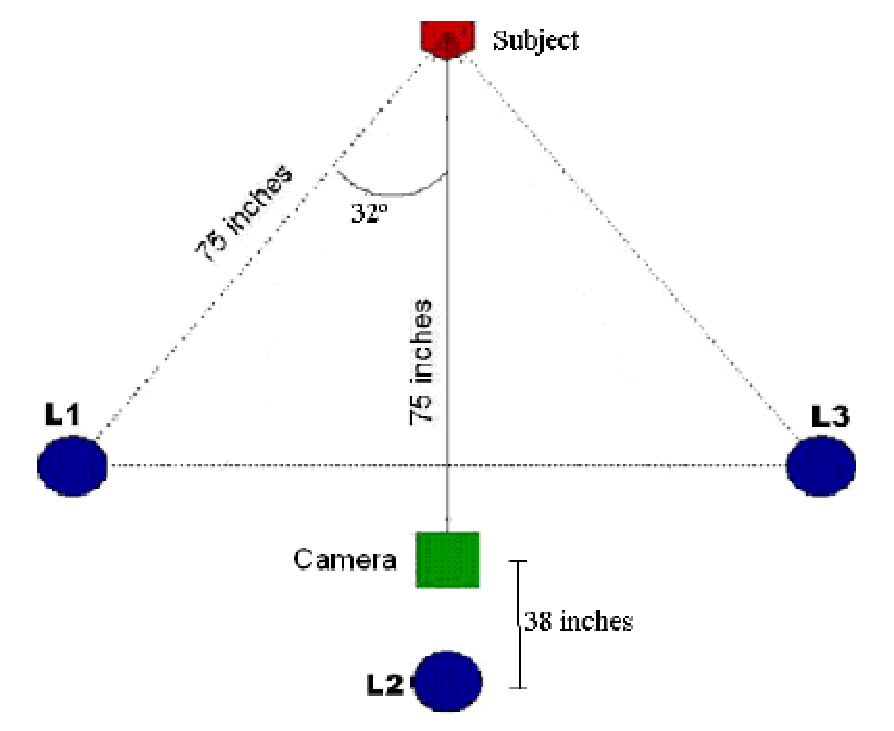
\includegraphics[scale=0.5]{fig01}
%  \caption{Write the figure caption here.}
%  \label{fig:pendulum}
%\end{figure}
%\end{verbatim}
%\begin{figure}
%\centering
%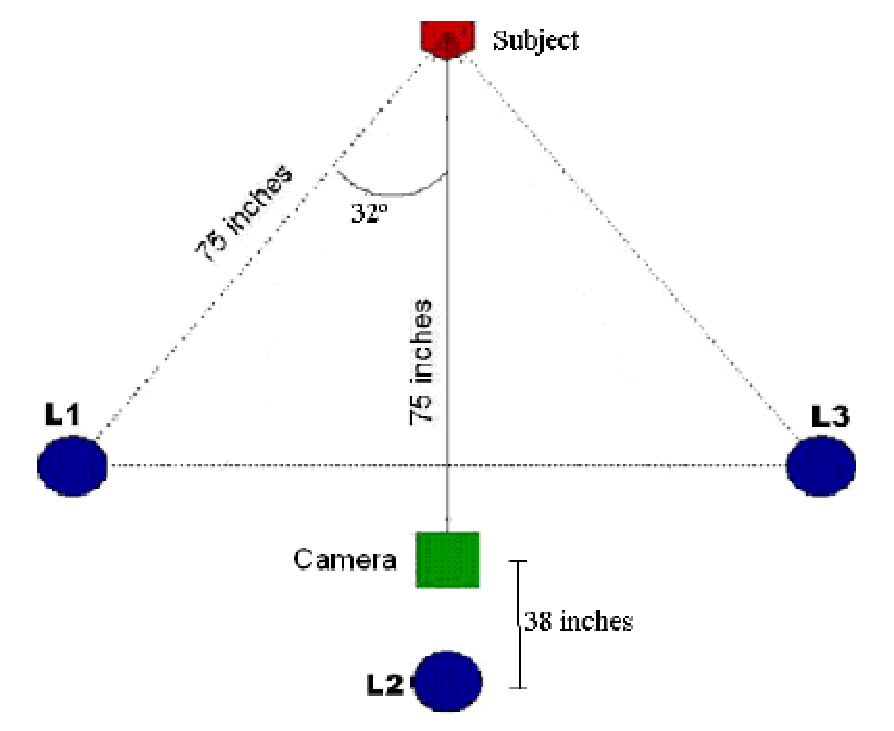
\includegraphics[scale=0.5]{fig01.pdf}
%\caption{Write the figure caption here.}
%\label{fig:pendulum}
%\end{figure}

%\subsection{And a table?}
%Just replace the text/values in the template table below 
%with your own. You can change the number of 
%lines/rows as necessary.
   
%\begin{table*}
%\centering
%\caption{Title of the table should be at the top}
%\begin{tabular}{|l|l|l|l|}
%\hline
%Column Name1    & Column Name2 & Column Name3 & Column Name4 \\
%\hline
%Parameter Name1 & Value        & Value        & Value        \\
%\hline
%Parameter Name2 & Value        & Value        & Value        \\
%\hline
%Parameter Name3 & Value        & Value        & Value        \\
%\hline
%\end{tabular}
%\end{table*}

%\subsection{Equations}
%Conventionally, in mathematical equations, variables and
%anything that represents a value appear in italics. 
%All equations should be numbered for easy referencing. 
%The number should appear at the right margin.
%\begin{eqnarray}
%S'_{\mathrm{pg}} = \frac{S_{\mathrm{pg}} - \mathrm{min}(S_{\mathrm{pG}})}
%  {\mathrm{max}(S_{\mathrm{pG}} - \mathrm{min}(S_{\mathrm{pG}}))}
%\end{eqnarray}
%In mathematical expressions 
%in running text "/" should be used
%for division (not a horizontal line).

%\section{Citations}
%Citations in the text can be made using\\[6pt]
%\verb+\citet{NewmanGirvan2004}+\\[6pt]
%for citation in running text like in 
%\citet{NewmanGirvan2004} or using\\[6pt]
%\verb+\citep{Vehlowetal2013,NewmanGirvan2004}+\\[6pt]
%for citation within parentheses like in 
%\citep{Vehlowetal2013,NewmanGirvan2004}.

%Please use the actual \verb+\cite+ command in the text.
%Also, please double-check the \verb+\citep+ command.

%\section{Reference style}
%You can include the references in the main text file in \LaTeX
%format. Alternately, you can include a separate bibliography
%file (refs.bib in this example) and run the following set of 
%commands:
%\begin{verbatim}
%==================

%pdflatex myfile.tex

%bibtex myfile (no extension in this line!)

%pdflatex myfile.tex

%pdflatex myfile.tex

%==================
%\end{verbatim}

%\section{A sample entry in the bibliography file}
%{\fontsize{7.5pt}{9.6pt}\selectfont
%\begin{verbatim}
%==================

%@ARTICLE{NewmanGirvan2004,
%  author  = {Newman, M. E. J. and Girvan, M.},
%  title   = {Finding and evaluating community 
%               structure in networks},
%  journal = {Phys. Rev. E.},
%  volume  = {69},
%  number  = {21},
%  year    = {2004},
%  pages   = {026113}
%}

%==================
%\end{verbatim}
%}

\section{Acknowledgments}

The RINEX data used in this paper were obtained from the Trans-boundary, Land and Atmosphere Long-term Observational and Collaborative Network (TLALOCNet, \citet{Cabral-Cano:2018}), operated by the Servicio de Geodesia Satelital (SGS) at the Instituto de Geofísica-Universidad Nacional Autónoma de México (UNAM) in collaboration with UNAVCO Inc. 

We are deeply grateful to all personnel from SGS, SSN and UNAVCO for station installation, maintenance, data acquisition, IT support and data curation and distribution for these networks and in particular to the following individuals and institutions, and those whose hard field work and resourcefulness were central to the success of this project: Bill Douglass, Neal Lord and Bill Unger at UW-Madison, Oscar Diaz-Molina and Luis Salazar-Tlaczani at SGS, John Galetzka, Adam Wallace, Shawn Lawrence, Sean Malloy and Chris Walls at UNAVCO, Jesus Pacheco-Martínez at Universidad Autónoma de Aguascalientes, Bertha Marquez-Azúa and personnel at the Universidad de Guadalajara at campus Guadalajara, Mascota and Ameca, Protección Civil de Jalisco, Universidad de Colima at campus Colima and campus El Naranjo and Centro de Geociencias, Centro de Ciencias de la Atmosfera Instituto de Biología Estacion Chamela at UNAM.
TLALOCNet, SSN-TLALOCNet and other GPS related operations from SGS are supported by CONACyT projects 253760, 256012 and 2017-01-5955, UNAM-PAPIIT projects IN104213, IN111509, IN109315-3, IN104818-3, NSF grant 2025104, NASA-ROSES grant NNX12AQ08G and supplemental support from UNAM-Instituto de Geofísica. UNAVCO's initial support for TLALOCNet (some of its stations now part of the GAGE Facility-NOTA) was performed under EAR-1338091 and is currently supported by NSF and NASA under NSF Cooperative Agreement EAR-1724794.

Also we are grateful with the Direcci\'on General de Asuntos Acad\'emicos (DGAPA) of the Universidad Nacional Aut\'onoma de M\'exico and the Programa de Becas Posdoctorales for funding this project.

%% Bibliography
%% Author year style
\bibliographystyle{model5-names}
\biboptions{authoryear}
\bibliography{bibliography}

\end{document}

%%

